\documentclass[14pt,a4paper]{scrartcl}
\usepackage[left=1.5cm,right=1.5cm,
    top=1.5cm,bottom=1cm,bindingoffset=0cm]{geometry}

\usepackage[T1,T2A]{fontenc}
\usepackage[utf8]{inputenc}
\usepackage[english,russian,ukrainian]{babel}
\usepackage{tabularx}
\usepackage{amssymb}
\usepackage{color}
\usepackage{amsmath}
\usepackage{mathrsfs}
\usepackage{listings}
\usepackage{graphicx}
\graphicspath{ {./images/} }
%\usepackage{draftwatermark} не будет лезть на картинки
\usepackage[printwatermark]{xwatermark}%будет лезть на картинки
\usepackage{lipsum}
\usepackage{xcolor}
\usepackage{tikz}

 \usepackage{csvsimple}
 \usepackage{supertabular}
\usepackage{pdflscape}
\usepackage{fancyvrb}
\usepackage{comment}



\begin{document}
\pagecolor{white}
\begin{titlepage}
  \begin{center}
    \large
    Національний технічний університет України \\ "Київський політехнічний інститут імені Ігоря Сікорського"
     
       
    Факультет Електроніки
     
    Кафедра мікроелектроніки
    \vfill
      
    \textsc{ЗВІТ}\\
     
    {\Large Про виконання практичної роботи №3\\
      з дисципліни: «Твердотільна електроніки-1»\\[1cm]
    }
  \bigskip
\end{center}
\vfill
 
\newlength{\ML}
\settowidth{\ML}{«\underline{\hspace{0.4cm}}» \underline{\hspace{2cm}}}
\hfill
\begin{minipage}{1\textwidth}
Виконавець:\\
Студент 3-го курсу \hspace{4cm} $\underset{\text{(підпис)}}{\underline{\hspace{0.2\textwidth}}}$  \hspace{1cm}А.\,С.~Мнацаканов\\
\vspace{1cm}

Превірив: \hspace{6.1cm} $\underset{\text{(підпис)}}{\underline{\hspace{0.2\textwidth}}}$  \hspace{1cm}Л.\,М.~Королевич\\

\end{minipage}

\vfill

\begin{center}
2020
\end{center}
\end{titlepage}
%---------------------------------------------------------------------------------------------------------------------------------------------------------------------------------

\begin{center}\textbf{1. Завдання}\\ \end{center}

Побудувати графіки розподілу електричного поля, елеткричного потенціалу та енергетичні діаграми ідеалізованого p-n переходу. Розрахувати відстань між металургійною і реальною межами поділу pn переходу. Розрахунки і побудови робити в рівноважному стані, а також при двох прикладених зовнішній напругах: $(0,8)\cdot \varphi_0$ та $(-2)\cdot \varphi_0$ (побудови для всіх трьох випадків робити на одному графіку з однаковим масштабом).\\
%---------------------------------------------------------------------------------------------------------------------------------------------------------------------------------


\newpage
\begin{center}\textbf{2. Розрахунки та побудова графіків}\\ \end{center}


Для того щоб побудувати графік розподілу електричного поля я буду користуватися формулами які я отримав у практичній роботі №2, ось перша пара:
\begin{align}
E_p(x) = \dfrac{qN'_A}{2\varepsilon\varepsilon_0} \cdot (x^2-l_p^2)\\
E_n(x) = \dfrac{qN'_D}{2\varepsilon\varepsilon_0}\cdot(x^2-l_n^2)
\end{align}

\begin{center}
\begin{figure}[h]
\center{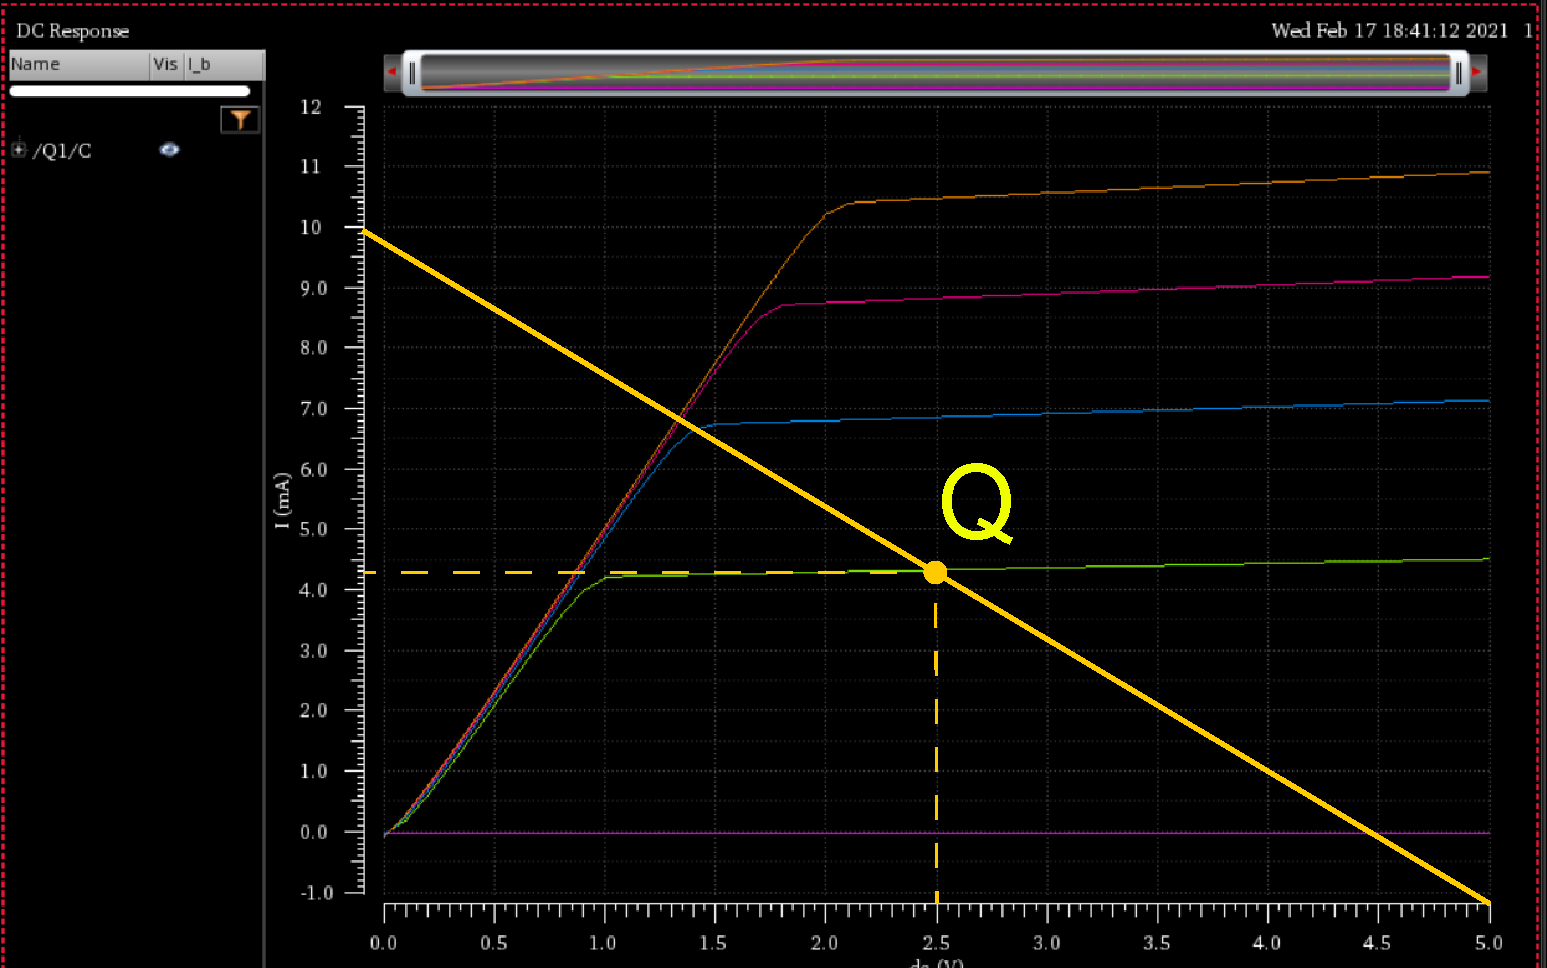
\includegraphics{1.pdf}}
\caption{Графіки розподілу електричного поля}
\label{ris:image1}
\end{figure}
\end{center}



\newpage
Наступні графіки (Рис. \ref{ris:image2}) були побудовані з використанням формул, які теж були виведені в попередній роботі:
\begin{align}
\varphi_p(x)=\dfrac{qN'_A}{6\varepsilon\varepsilon_0} \cdot (3l_p^2x-x^3+2l_p^3)\\
\varphi_n(x)= \varphi_0+\dfrac{qN'_D}{6\varepsilon\varepsilon_0}\cdot (3l_n^2x-x^3-2l_n^3)
\end{align}

\begin{center}
\begin{figure}[h]
\center{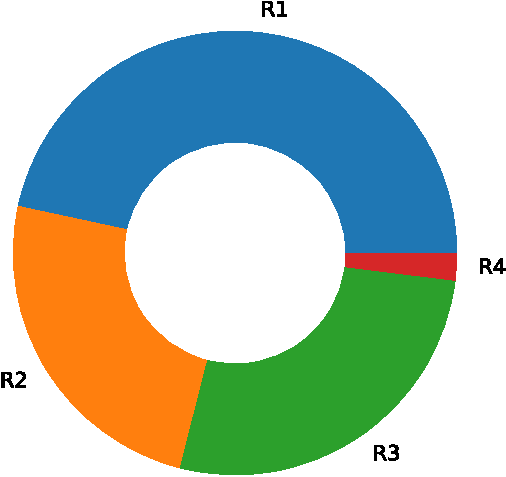
\includegraphics{2.pdf}}
\caption{Графіки розподілу електричного потенціалу}
\label{ris:image2}
\end{figure}
\end{center}

\newpage
\clearpage
Для того щоб знайти функцію за допомогою якої можна описати енергетичну діаграму p-n переходу я знайшовши $E_{F_{i}}$ за формулою:

Для того щоб отримати схожу діаграму як в книжці та зробити все як прийнято, тобто зона провідності зверху а валентна зона знизу, то я до функції що описує потенціал приставив знак мінус, тобто перевеннув їх та оримав графіки як на Рис. \ref{ris:image5}. Також для знаходження $\delta$ я знайшов положення рівня Фермі та його точку перетину ідеалізованим графіком, відстань від цієї точки до нуля і буде відстань між металургійною і реальною межами поділу pn переходу. 
\begin{equation}
E_{F_{i}} = \dfrac{E_{C} + E_V}{2},\\
\end{equation}

 де  $E_C=0.7099$ та $E_V=-0.71$  які я заздалегідь визначив зі своїх графіків підставивши отримав наступне:
 
 \begin{equation}
E_{F_{n}} = E_{F_{i}} - k\cdot T\cdot ln\left(\dfrac{N_D}{n_i} \right),\\
\end{equation}
де $k = 8.617333262\cdot10^{-5} eB\cdot K^{-1}$, T = 300 K, $N'_D = 3.8\cdot10^{18}$, $n_i = 1.79\cdot10^6$


\begin{center}
\begin{figure}[h]
\center{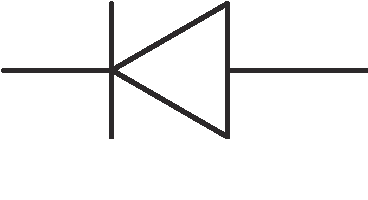
\includegraphics[height=10cm, width=12cm]{1.1.png}}
\caption{Енергетична діаграма ідеалізованого p-n переходу (з книги)}
\label{ris:image3}
\end{figure}
\end{center}

\begin{center}
\begin{figure}[h]
\center{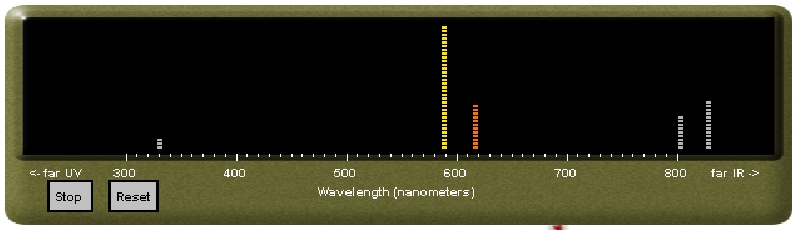
\includegraphics{3.pdf}}
\caption{Енергетична діаграма ідеалізованого p-n переходу}
\label{ris:image4}
\end{figure}
\end{center}

\begin{center}
\begin{figure}[h]
\center{\includegraphics{3.1.pdf}}
\caption{Енергетичні діаграми ідеалізованого p-n переходу}
\label{ris:image5}
\end{figure}
\end{center}


\clearpage
\newpage
\begin{center}\textbf{4. Таблиці контрольних величин}\\ \end{center}


Графiки розподiлу електричного поля\\

\begin{tabular}{ | c | c | c | }
\hline
& p, см & n, см  \\ \hline
рівноважний стан & -0.000986104 & 7.502e-05 \\
U = (0,8)$\cdot\varphi_0$ & -0.00055042 & 4.188e-05 \\
U = (-2)$\cdot\varphi_0$ & -0.00135746 & 0.00010328 \\
\hline
\end{tabular}

Графіки розподілу електричного потенціалу\\

\begin{tabular}{ | c | c | c | }
\hline
& p, см & n, см  \\ \hline
рівноважний стан & -0.000986104 & 7.5e-05 \\
U = (0,8)$\cdot\varphi_0$ & -0.0005504 & 4.188e-05 \\
U = (-2)$\cdot\varphi_0$ & -0.001357463 & 0.00010328 \\
\hline
\end{tabular}


Енергетичні діаграми ідеалізованого p-n переходу\\

\begin{tabular}{ | c | c | c | c | }
\hline
			      		& p, см 		 & n, см  		&  висота потенціального бар'єру \\ \hline
рівноважний стан 		& -0.000986104 & 7.5e-05  	&\\
U = (0,8)$\cdot\varphi_0$ & -0.000550 	 & 4.188e-05 	& \\
U = (-2)$\cdot\varphi_0$   & -0.00135746 	 & 0.00010328  & \\
\hline
\end{tabular}



\end{document}
